\subsection{Storia}
Questo sistema operativo fu inizialmente creato dalla \textit{Android inc.} ma venne quasi subito acquistato da \textit{Google} e rilasciato col nome di \textit{Android Open Source Project} (AOSP) nel 2007 \cite{androiden}. Parallelamente a questo evento venne fondata la \textit{Open Handset Alliance} (OHA), un consorzio dedicato allo sviluppo e distribuzione di Android. Il software fu rilasciato sotto licenza \textit{Apache} (gratis, libera e open source). La OHA è formata da diverse case produttrici di hardware, software e telecomunicazioni come \textit{Google}, \textit{Intel}, \textit{NVIDIA}, \textit{Qualcomm}, \textit{Motorola}, \textit{HTC}, \textit{T-Mobile}, ecc. \cite{androiden} Il suo obbiettivo è quello di sviluppare tecnologie che permettono di abbassare nettamente i tempi e i costi della creazione e distribuzione di dispositivi mobili e relativi servizi.\\
\\
Android crebbe in modo molto rapido ed ancora oggi è supportato con frequenti aggiornamenti di sicurezza e nuove versioni. Quasi tutte hanno il nome di un cioccolatino, caramella o di un alimento inerente al mondo dei dolci e le iniziali di ognuna sono ordinate alfabeticamente in modo crescente. Nelle ultime versioni, come si può vedere dalla seguente tabella, questa particolarità si è persa.

%% per allungare il brodo posso aggiungere le principali innovazioni per ogni versione

\begin{center}
    
    \begin{tabular}{ll}
    \textit{Versione} & \textit{Nome} \\ [0.5ex]
    \cline{1-2}
       1.5 & Cupcake\\ [0.5ex]
       1.6 & Donut\\ [0.5ex]
       2.0 & Éclair\\ [0.5ex]
       2.2 & Froyo\\ [0.5ex]
       2.3 & Gingerbread\\ [0.5ex]
       4.0 & Ice Cream Sandwich\\ [0.5ex]
       4.1 & Jelly Bean\\ [0.5ex]
       4.4 & KitKat\\ [0.5ex]
       5.0 & Lollipop\\ [0.5ex]
       6.0 & Marshmallow\\ [0.5ex]
       7.0 & Nougat\\ [0.5ex]
       8.0 & Oreo\\ [0.5ex]
       9 & Pie\\ [0.5ex]
       10 & 10\\ [0.5ex]
       11 & 11\\ [0.5ex]
    \end{tabular}
    \captionof{table}{Tabella riassuntiva di tutte le versioni di Android}
\end{center}

Il primo dispositivo commercializzato che utilizzava Android fu l'\textit{HTC Dream} (2008) \cite{androidwikipedia}, noto anche con il nome di \textit{T-Mobile G1} (negli Stati Uniti e in alcune parti dell'Europa) o Era G1 (in Polonia). Montava un processore Qualcomm \textit{MSM7201A ARM11} a 528 MHz, 256 MB di memoria interna, espandibile fino a 16 GB con microSD, 192 MB di RAM e una batteria a ioni di litio (rimovibile) da 1150 mAh. Era dotato di uno schermo da 3,2 pollici LED con touchscreen capacitivo ad una risoluzione di 320x480 pixel. La scocca portante era completamente in plastica ed aveva una tastiera QWERTY fisica.

Successivamente, divenne una pratica comune per Google utilizzare il lancio dei suoi nuovi dispositivi come base per le nuove versioni di Android: un esempio è il \textit{Nexsus 5} che fu introdotto nel 2013 \cite{androidwikipedia} con \textit{KitKat} (la allora nuovissima versione di Android), il \textit{Nexsus 6} con \textit{Lollipop} o il \textit{Pixel} con \textit{Nougat 7.1}.

\begin{figure}[H]
  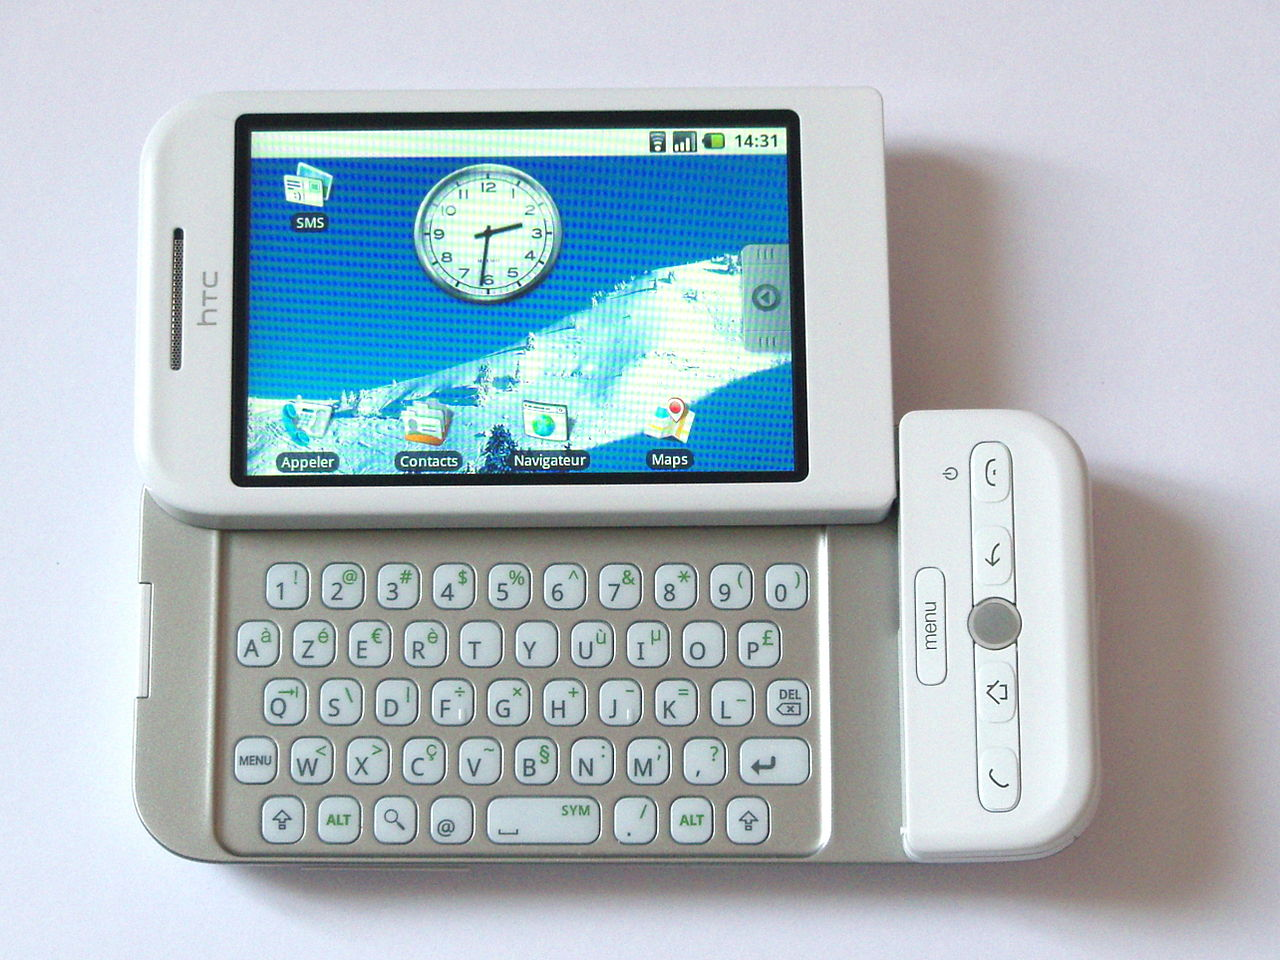
\includegraphics[scale=0.27]{android/imgs/htc_dream.jpeg}
  \caption{HTC Dream}
  Questa immagine \cite{androidwikipedia} mostra un esemplare di HTC Dream nella sua colorazione bianca con tastiera AZERTY.
\end{figure}